% Assignment 1 - Basic Matrix Multiplication in Different Languages
% Compile with pdfLaTeX (e.g. Overleaf). Figures are in the figures/ folder.
\documentclass[11pt,a4paper]{article}
\usepackage[margin=2.2cm]{geometry}
\usepackage[T1]{fontenc}
\usepackage[utf8]{inputenc}
\usepackage{lmodern}
\usepackage{graphicx}
\usepackage{booktabs}
\usepackage{float}
\usepackage{needspace} % \needspace{h}: start a new page unless h of space is left,
                       % so a heading and its intro text stay with their table/figure
\usepackage{amsmath}
\usepackage{mathtools}
\usepackage{listings}
\usepackage{xcolor}
\usepackage[hidelinks]{hyperref}

\lstset{basicstyle=\ttfamily\small, frame=single, columns=fullflexible,
        keywordstyle=\color{blue!60!black}\bfseries}

\title{\textbf{Assignment 1: How Matrix Size Affects the Runtime and Memory\\
of Basic Matrix Multiplication in Python, Java and C}}
\author{Daniel Perdomo Medina\\
Big Data --- Grado en Ciencia e Ingenier\'ia de Datos, ULPGC, 2026--2027}
\date{October 2026}

\begin{document}
\maketitle

% ---------------------------------------------------------------------------
\begin{abstract}
\noindent
This study asks how the matrix size $n$ affects the runtime and the memory use of
the same textbook $O(n^3)$ matrix multiplication written in Python, Java and C.
The three implementations use the same triple loop (i--j--k order), the same
float64 inputs read from shared files, and they were validated against known
answers and against NumPy before benchmarking. On one laptop (Intel Core i7-13620H,
Windows 11), every configuration was run five times after warm-up, and the median,
the interquartile range and the peak process memory were recorded for
$n = 100, 200, \dots, 3200$. Runtime grew by roughly $8$--$12\times$ per doubling of
$n$ while the data fitted in the CPU caches, as the cubic model predicts, and grew
faster for larger matrices. C was the fastest implementation at every tested size;
Java was $1.2$--$1.6\times$ slower than C up to $n = 800$ but $6.5\times$ slower at
$n = 1600$; CPython was $87$--$162\times$ slower than C. The largest sizes that
finished within a 600\,s budget were $n = 1600$ for C and Java and $n = 800$ for Python.
These conclusions apply only to these implementations, settings and this machine.
\end{abstract}

% ---------------------------------------------------------------------------
\section{Introduction and objective}

Matrix multiplication is a basic building block of data science and machine learning,
and its cost grows quickly with the size of the matrices. Before studying optimised,
sparse, parallel and distributed versions in later assignments, this first study
establishes a \emph{baseline}: the simplest algorithm written in three widely used
languages that execute code in very different ways (an interpreter, a JIT-compiling
virtual machine and an ahead-of-time compiler).

\paragraph{Research question.} \emph{How does the matrix size $n$ affect the runtime
and the memory use of the basic triple-loop matrix multiplication implemented in
Python, Java and C on one fixed machine?}

The factor that changes is $n$ (side length of the $n\times n$ square matrices) and the
implementation language; the outcomes are the multiplication time and the peak memory
of the process.

\paragraph{Hypotheses (predictions made before measuring).}
\begin{itemize}
  \item[H1] Runtime grows approximately as $n^3$, i.e.\ about $8\times$ every time
        $n$ doubles, for all three implementations.
  \item[H2] C and Java will be within a small factor of each other, and CPython will be
        one to two orders of magnitude slower, because it interprets every operation.
  \item[H3] Memory grows approximately as $n^2$ (three $n\times n$ matrices), with a
        constant runtime overhead that is largest for the JVM and with a larger
        per-element cost in Python, where every number is an object.
\end{itemize}

% ---------------------------------------------------------------------------
\section{Background and references}

\paragraph{Algorithm.} For $C = AB$ with $A, B \in \mathbb{R}^{n\times n}$, each element
is the dot product $c_{ij} = \sum_{k=0}^{n-1} a_{ik} b_{kj}$. Computing $n^2$ elements,
each with $n$ multiply--add operations, costs exactly $n^3$ multiplications and $n^3$
additions, so the work is $\Theta(n^3)$ \cite{golub}. Asymptotically faster algorithms
exist (e.g.\ Strassen) but are out of scope; the assignment requires the straightforward
triple loop.

\paragraph{Memory hierarchy.} The time of a multiply--add depends on where its operands
are: registers and caches are much faster than main memory \cite{drepper}. In the i--j--k
order, the inner loop reads a \emph{row} of $A$ (consecutive addresses, cache friendly)
but a \emph{column} of $B$ (addresses $8n$ bytes apart, one cache line per element).
When the matrices no longer fit in the caches, the cost per operation is expected to rise,
so measured times can grow faster than the pure $n^3$ model.

\paragraph{Execution models.} C is compiled ahead of time to machine code by GCC.
Java is compiled to bytecode, which the HotSpot JVM first interprets and then
compiles to machine code just-in-time (JIT) once a method is ``hot''; this is why
warm-up runs are needed \cite{georges}. CPython interprets bytecode and represents every
float as a heap object, so every arithmetic operation involves type dispatch and object
handling.

\paragraph{Benchmarking practice.} Repeated measurements, warm-up, and robust summaries
(median, interquartile range) are recommended because single measurements of modern
systems are noisy \cite{georges, kalibera}.

% ---------------------------------------------------------------------------
\needspace{0.3\textheight}
\section{Methodology}

\subsection{Implementations}
The three programs implement exactly the same loop (Listing~\ref{lst:kernel}), with a
local accumulator and the same i--j--k order, using 64-bit IEEE-754 floating point
(\texttt{double} in C and Java, \texttt{float} in Python). No optimised library is used
inside any measured kernel.

\needspace{12\baselineskip}
\begin{lstlisting}[language=C, caption={Kernel shared by the three implementations (C version).}, label={lst:kernel}]
for (int i = 0; i < n; i++)
    for (int j = 0; j < n; j++) {
        double sum = 0.0;
        for (int k = 0; k < n; k++)
            sum += A[i * n + k] * B[k * n + j];
        C[i * n + j] = sum;
    }
\end{lstlisting}

\noindent\textbf{Storage layouts (unavoidable language differences).}
\begin{itemize}
  \item \textbf{C}: one contiguous \texttt{malloc} block of $n^2$ doubles per matrix,
        row-major (\texttt{A[i*n+k]}); 8 bytes per element.
  \item \textbf{Java}: \texttt{double[n][n]}, an array of $n$ row arrays. Each row is
        contiguous, but rows are separate heap objects, and each access \texttt{B[k][j]}
        first loads the reference to row \texttt{k} and is bounds-checked.
  \item \textbf{Python}: a list of $n$ lists. Each list stores 8-byte pointers to
        separate \texttt{float} objects (24 bytes each in CPython), so about 32 bytes
        per element, possibly scattered in memory.
\end{itemize}

\subsection{Inputs}
For every $n$, the matrices $A$ and $B$ were generated once with NumPy
(\texttt{default\_rng(2026 + n)}, uniform values in $[-1, 1)$) and saved as binary files
of little-endian float64 values in row-major order. All three programs read the same
files, so they multiply exactly the same logical matrices and no cross-language random
generator is involved. Declared size sequence: $n = 100, 200, 400, 800, 1600, 3200$;
doubling $n$ makes the expected cubic growth easy to check ($\times 8$ per step).

\needspace{0.25\textheight}
\subsection{Environment and fixed settings}
\begin{table}[H]
\centering\small
\begin{tabular}{ll}
\toprule
Item & Value \\
\midrule
CPU & Intel Core i7-13620H: 6 performance + 4 efficiency cores, 16 logical CPUs \\
    & 24\,MB shared L3 cache \cite{intel} \\
RAM / OS & 16\,GB / Windows 11 Home (build 26200), laptop plugged in \\
C & GCC 16.2.0 (MinGW-w64 UCRT), flags \texttt{-O2 -std=c11 -static} \\
Java & Oracle JDK 24.0.1, HotSpot 64-bit Server VM, flag \texttt{-Xmx3g} \\
Python & CPython 3.11.9 (standard library only in the kernel) \\
Helper tools & NumPy 2.2.0 (inputs, reference), psutil 6.1.0 (memory), pandas, matplotlib \\
Threads & all kernels single-threaded; no numerical library inside the kernels \\
\bottomrule
\end{tabular}
\caption{Machine and toolchain. These settings were fixed for all runs.}
\end{table}

The flag \texttt{-O2} is GCC's standard optimisation level; it was kept fixed and no
architecture-specific (\texttt{-march=native}) or unsafe floating-point
(\texttt{-ffast-math}) flags were used, so the compiler may not reorder the
floating-point sum. \texttt{-static} only avoids a run-time DLL dependency. The JVM
used its default JIT (tiered compilation) and garbage collector (G1); \texttt{-Xmx3g}
caps the heap below the memory budget.

Because the CPU is hybrid, a first exploratory run (kept in
\texttt{results/exploratory\_unpinned/}) showed large run-to-run variation, e.g.\ five
consecutive Python runs at $n = 200$ ranged from 0.67\,s to 2.95\,s, consistent with the
operating system moving the process between fast and slow cores. In the final run every
benchmark process was therefore pinned to the performance cores (logical CPUs 0--11) with
high priority.

\subsection{Timing protocol}
\begin{itemize}
  \item \textbf{Timed region}: only the multiplication kernel. Reading the input files
        and allocating the result matrix happen \emph{before} the timer starts.
  \item \textbf{Timers}: monotonic clocks: \texttt{clock\_gettime(CLOCK\_MONOTONIC)} in C,
        \texttt{System.nanoTime()} in Java, \texttt{time.perf\_counter()} in Python.
  \item \textbf{Warm-up}: C 1 run, Python 1 run (caches, page faults), Java 2 runs (JIT
        compilation). Warm-up runs are recorded in the raw data but excluded from the
        statistics.
  \item \textbf{Repetitions}: 5 measured runs per configuration, all in the same process.
        Reported: median and interquartile range (IQR $= Q_3 - Q_1$), plus min and max.
  \item \textbf{Result consumption}: after each run the program sums all elements of $C$
        (checksum) and prints it, so the computation cannot be skipped by the compiler;
        each checksum is compared with NumPy's result (relative tolerance $10^{-9}$).
\end{itemize}

\subsection{Memory measurement}
The metric is the \textbf{peak resident memory of the whole process} (on Windows, the
\emph{peak working set}), read with psutil \cite{psutil} every 10\,ms by the benchmark script. It
includes the language runtime (JVM, interpreter) and all data, not only the matrices.
As a reference, the raw storage of three float64 matrices is $3 \times 8n^2$ bytes.

\subsection{Budgets and limits}
Before the large tests, a budget was declared per configuration (one language and one
$n$, including warm-ups): \textbf{600\,s of wall time} and \textbf{4096\,MB of memory}.
A configuration exceeding a budget is killed and recorded as TIMEOUT or MEMORY\_LIMIT;
larger sizes of that language are then recorded as SKIPPED. No execution time is invented
for them.

\subsection{Correctness checks}
Before benchmarking, each implementation multiplied four test cases and wrote its result
to a file:
(1) a hand-computed $2\times 2$ case $\begin{psmallmatrix}1&2\\3&4\end{psmallmatrix}
\begin{psmallmatrix}5&6\\7&8\end{psmallmatrix}=\begin{psmallmatrix}19&22\\43&50\end{psmallmatrix}$;
(2) $A \cdot I = A$ with $n = 37$; (3) $A \cdot 0 = 0$ with $n = 37$ (all three required
\emph{exact} equality); and (4) random $A, B$ with $n = 100$ compared with NumPy's
\texttt{A @ B}, accepted if $|c - c_{\text{ref}}| \le 10^{-9} + 10^{-9}|c_{\text{ref}}|$
for every element. The tolerance is justified by the rounding-error bound of a dot
product, $|\hat{c}-c| \le \gamma_n \sum_k |a_{ik} b_{kj}|$ with
$\gamma_n \approx n u$ and $u \approx 1.1\times 10^{-16}$ \cite{higham}: for $n=100$
and values in $[-1,1)$ this is of order $10^{-13}$, far below $10^{-9}$, while an
indexing bug would produce errors of order $1$. NumPy sums in a different order (BLAS),
so tiny differences are legitimate.

% ---------------------------------------------------------------------------
\needspace{0.3\textheight}
\section{Results}

\subsection{Correctness}
All implementations passed all tests (Table~\ref{tab:correct}). The exact tests gave
zero error. In the random test the maximum difference from NumPy was
$5.3\times 10^{-15}$, and the three implementations produced \emph{bitwise identical}
matrices, as expected since they perform the same operations in the same order with
IEEE-754 doubles. During the benchmark, every checksum matched the NumPy reference.

\begin{table}[H]
\centering\small
\begin{tabular}{lrlcc}
\toprule
Test & $n$ & Criterion & Max abs.\ error (C, Java, Python) & Passed \\
\midrule
known $2\times2$ & 2 & exact & 0, 0, 0 & yes (all) \\
identity $A\cdot I$ & 37 & exact & 0, 0, 0 & yes (all) \\
zero $A\cdot 0$ & 37 & exact & 0, 0, 0 & yes (all) \\
random vs NumPy & 100 & rtol = atol = $10^{-9}$ & $5.3\times10^{-15}$ (each) & yes (all) \\
\bottomrule
\end{tabular}
\caption{Correctness tests (\texttt{results/raw/correctness.csv}).}
\label{tab:correct}
\end{table}

\needspace{0.5\textheight}
\subsection{Runtime}
Table~\ref{tab:runtime} summarises the five measured runs of every configuration that
finished within budget; Figure~\ref{fig:runtime} shows the medians on log--log axes.

\begin{table}[H]
\centering\small
\begin{tabular}{lrrrrrr}
\toprule
Lang. & $n$ & Median (s) & IQR (s) & IQR/median & ns per mult-add & Growth vs $n/2$ \\
\midrule
C      & 100  & 0.0002703 & 0.000011 & 4.0\% & 0.27 & --- \\
C      & 200  & 0.002717  & 0.000091 & 3.3\% & 0.34 & 10.1$\times$ \\
C      & 400  & 0.03216   & 0.00018  & 0.6\% & 0.50 & 11.8$\times$ \\
C      & 800  & 0.3357    & 0.0026   & 0.8\% & 0.66 & 10.4$\times$ \\
C      & 1600 & 4.122     & 0.23     & 5.5\% & 1.01 & 12.3$\times$ \\
\midrule
Java   & 100  & 0.0004409 & 0.0000037 & 0.8\% & 0.44 & --- \\
Java   & 200  & 0.003361  & 0.000028 & 0.8\% & 0.42 & 7.6$\times$ \\
Java   & 400  & 0.05294   & 0.0088   & 16.6\% & 0.83 & 15.8$\times$ \\
Java   & 800  & 0.4976    & 0.058    & 11.6\% & 0.97 & 9.4$\times$ \\
Java   & 1600 & 26.79     & 1.9      & 7.0\% & 6.54 & 53.8$\times$ \\
\midrule
Python & 100  & 0.03706   & 0.0014   & 3.7\% & 37.06 & --- \\
Python & 200  & 0.3091    & 0.0034   & 1.1\% & 38.64 & 8.3$\times$ \\
Python & 400  & 2.803     & 0.029    & 1.0\% & 43.80 & 9.1$\times$ \\
Python & 800  & 54.30     & 2.2      & 4.1\% & 106.06 & 19.4$\times$ \\
\bottomrule
\end{tabular}
\caption{Multiplication time, 5 measured runs per row (warm-ups excluded).
``ns per mult-add'' $=$ median$/n^3$; a constant value means perfect cubic scaling.
Source: \texttt{results/tables/runtime\_summary.csv}.}
\label{tab:runtime}
\end{table}

\begin{figure}[H]
\centering
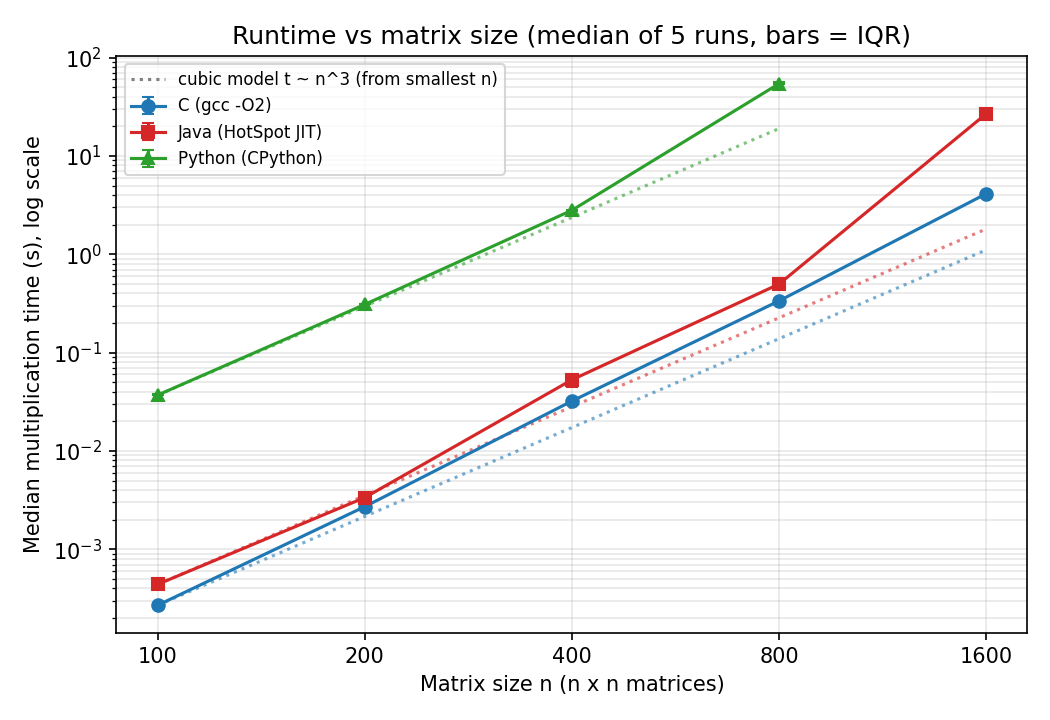
\includegraphics[width=0.78\textwidth]{figures/fig1_runtime_vs_n.png}
\caption{Median multiplication time versus $n$ (log--log). Error bars show the IQR
(mostly smaller than the markers). Dotted lines extrapolate each language's smallest-$n$
time with the cubic model $t \propto n^3$.}
\label{fig:runtime}
\end{figure}

\needspace{0.45\textheight}
Ratios of medians with respect to C: Java/C $= 1.6, 1.2, 1.6, 1.5, 6.5$ and
Python/C $= 137, 114, 87, 162$ for $n = 100, 200, 400, 800, (1600)$ respectively.
Fitting $t = a n^b$ to all completed sizes gives $b = 3.47$ (C), $3.90$ (Java) and
$3.47$ (Python). Figure~\ref{fig:perop} shows the cost per inner-loop operation.

\begin{figure}[H]
\centering
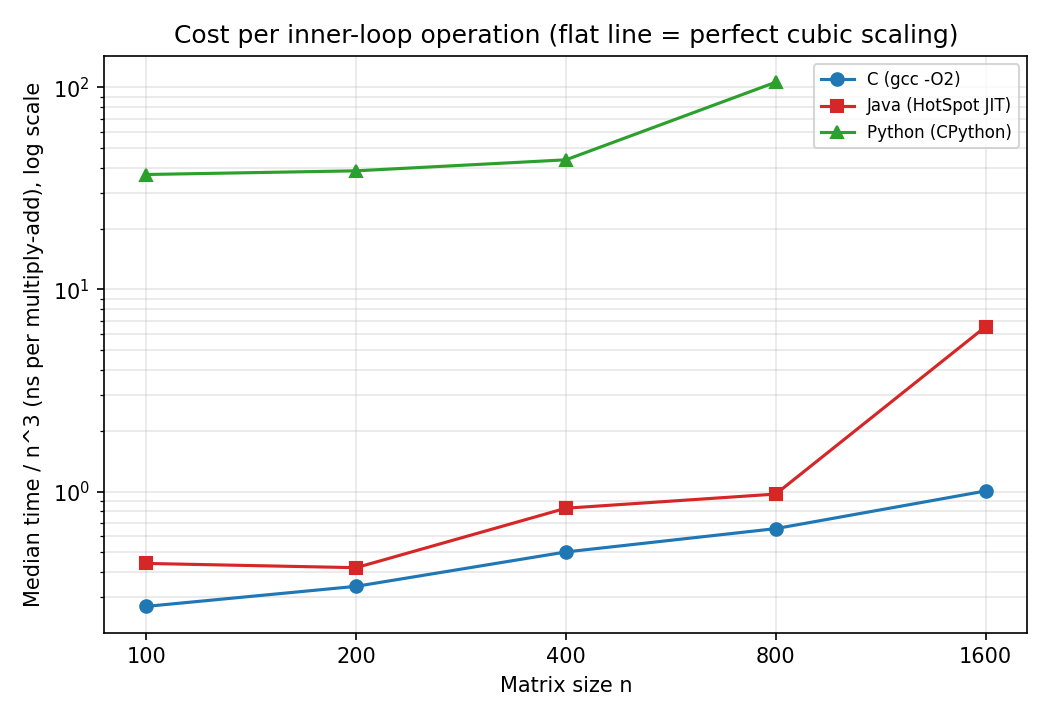
\includegraphics[width=0.72\textwidth]{figures/fig2_time_per_operation.png}
\caption{Median time divided by $n^3$ (nanoseconds per multiply--add). A flat line would
mean exact cubic scaling; an increasing line means each operation becomes more expensive
as the matrices grow.}
\label{fig:perop}
\end{figure}

\paragraph{Warm-up.} For Java, the first warm-up run was $5.7\times$ ($n=100$) and
$2.4\times$ ($n=200$) slower than the measured median, consistent with the JIT compiling
the kernel during the first runs. From $n = 400$ the ratio was close to 1, since the JIT
compiles the loop early inside the (longer) first run. For C and Python the first run was
within 6\% of the median (27\% for C at $n = 100$, where a run lasts 0.3\,ms).

\needspace{0.25\textheight}
\subsection{Memory}

\begin{table}[H]
\centering\small
\begin{tabular}{rrrrr}
\toprule
$n$ & C (MB) & Java (MB) & Python (MB) & $3\times 8n^2$ bytes (MB) \\
\midrule
100  & 9.1  & 43.0  & 16.5 & 0.23 \\
200  & 9.0  & 46.5  & 20.3 & 0.92 \\
400  & 11.8 & 52.5  & 33.8 & 3.66 \\
800  & 22.8 & 75.0  & 89.6 & 14.65 \\
1600 & 66.7 & 198.4 & ---  & 58.59 \\
\bottomrule
\end{tabular}
\caption{Peak resident memory (peak working set) of the whole process, measured with
psutil; MB $= 2^{20}$ bytes. Source: \texttt{results/tables/memory\_summary.csv}.}
\label{tab:memory}
\end{table}

\begin{figure}[H]
\centering
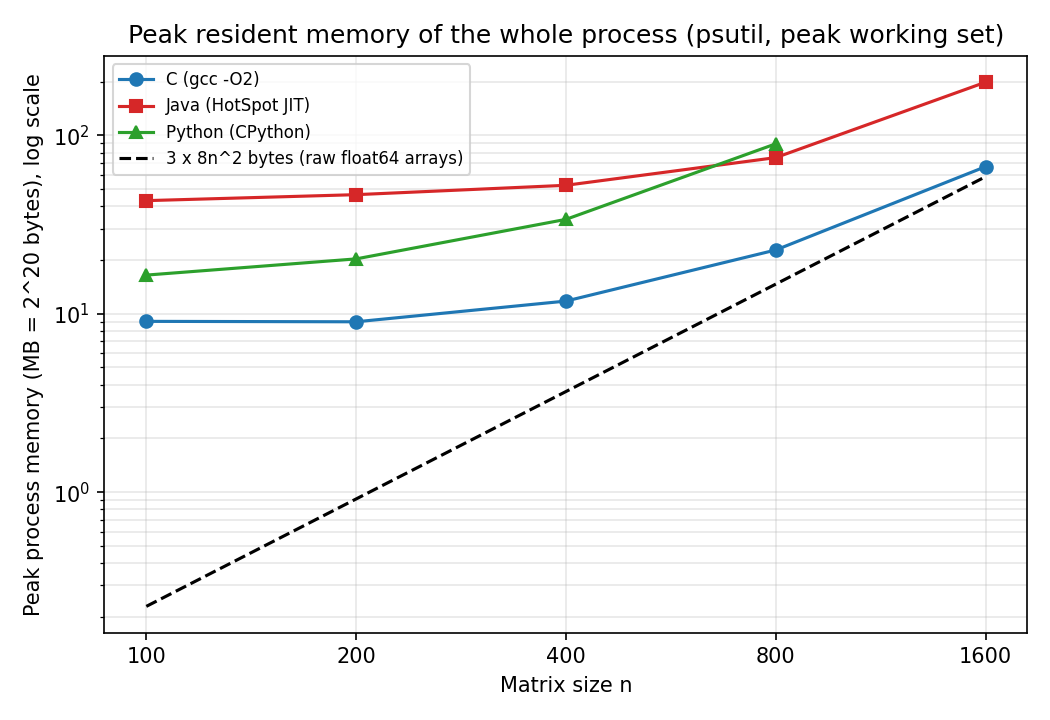
\includegraphics[width=0.72\textwidth]{figures/fig3_memory_vs_n.png}
\caption{Peak process memory versus $n$ (log--log). The dashed line is the raw storage of
three float64 matrices.}
\label{fig:memory}
\end{figure}

\needspace{0.22\textheight}
\subsection{Limits}

\begin{table}[H]
\centering\small
\begin{tabular}{lccc}
\toprule
Language & Largest feasible $n$ & First size over budget & Outcome at larger sizes \\
\midrule
C      & 1600 & 3200 (TIMEOUT after 600\,s, peak 242.5\,MB) & --- \\
Java   & 1600 & 3200 (TIMEOUT after 600\,s, peak 491.2\,MB) & --- \\
Python & 800  & 1600 (TIMEOUT after 600\,s, peak 311.7\,MB) & 3200 SKIPPED \\
\bottomrule
\end{tabular}
\caption{Largest size that met the 600\,s / 4096\,MB budget. No configuration reached the
memory budget. Source: \texttt{results/raw/runs\_status.csv}.}
\label{tab:limits}
\end{table}

The timed-out configurations are not summarised, but the runs that completed before the
limit are kept in the raw data: at $n = 3200$ a single C multiplication took about
252\,s, at least $60\times$ the $n = 1600$ median (cubic model: $8\times$); a Java warm-up
run took 309\,s; and at $n = 1600$ one Python warm-up run took 336\,s.

% ---------------------------------------------------------------------------
\section{Discussion}

\paragraph{Answer to the question (H1).} While the data are small, the runtime follows
the cubic model closely: Python grows $8.3\times$ and $9.1\times$ per doubling up to
$n = 400$, and C and Java grow $7.6$--$12\times$ up to $n = 800$. The cost per operation
is not perfectly constant, however (Figure~\ref{fig:perop}): for C it increases smoothly
from 0.27\,ns to 1.01\,ns, so the fitted exponents ($b \approx 3.5$--$3.9$) are larger than
3. The cubic model counts operations correctly, but it ignores how expensive each
operation is, which depends on the memory system and on the machine.

\paragraph{Memory-layout effects.} The sharpest changes appear when the working data
outgrow the 24\,MB L3 cache. Three matrices of $n = 800$ take 14.6\,MB in C and Java, but
about $3 \times 32 \times 800^2 \approx 61$\,MB in Python; Python's cost per operation jumps
from 43.8\,ns to 106\,ns exactly at $n = 800$. At $n = 1600$ (58.6\,MB of raw data) the cost
per operation of Java jumps from 0.97\,ns to 6.5\,ns, whereas C, running the same loop on
the same inputs, increases only from 0.66\,ns to 1.01\,ns. Because the algorithm, inputs and
machine are the same, the most plausible cause is the storage layout: walking down a column
of B in C uses addresses with a constant stride inside one block, which the hardware can
predict, while in Java each step must first load a different row reference and the rows
are separate objects. C shows a similar cliff only one size later (about 252\,s at
$n = 3200$, $\geq 60\times$ the time at $n = 1600$). These explanations are consistent with
the evidence but were not confirmed with hardware counters (cache or TLB misses), so they
remain hypotheses.

\paragraph{Interpreter and runtime effects (H2).} H2 is supported. Up to $n = 800$ Java
is only $1.2$--$1.6\times$ slower than C: after JIT compilation both execute machine code,
and the remaining gap is consistent with bounds checks and the extra row indirection.
CPython is $87$--$162\times$ slower than C, because every \texttt{+} and \texttt{*} is
executed by the interpreter on boxed \texttt{float} objects, which costs about 37--44\,ns per
multiply--add instead of below 1\,ns. The JIT is also visible in Java's warm-up runs.

\paragraph{Memory (H3).} H3 is supported. The runtime overhead dominates for small $n$:
the JVM needs about 43\,MB before the matrices matter, Python about 16\,MB, C about 9\,MB.
For large $n$ the growth follows $n^2$. C's increase from $n=100$ to $1600$ (57.6\,MB)
matches the raw storage (58.4\,MB). Python's increase from $n=100$ to $800$ (73\,MB for
$1.92$ million elements) is about 40 bytes per element, i.e.\ about $5\times$ the 8 bytes
of a C double, as expected from pointer plus float object. Java at $n = 1600$ (198\,MB)
uses more than three times the raw storage; the JVM heap also holds the byte buffers used
while reading the input files until the garbage collector reclaims them, and the heap
grows in steps. Memory never limited the experiment: time did.

\paragraph{System effects and limitations.}
\begin{itemize}
  \item \textbf{One machine.} All results come from one laptop; with a hybrid CPU,
        unpinned runs were unreliable (Section 3.3), so pinning to performance cores was
        part of the protocol.
  \item \textbf{Sustained load.} A supplementary check (\texttt{results/raw/supplementary\_sustained\_load\_check.txt})
        ran the Python $n=800$ case four times in a row: 31.9, 40.9, 43.4 and 57.2\,s,
        independently of pinning. The time increases with sustained load, which is
        consistent with the laptop lowering its clock under sustained load (this CPU
        has a lower sustained than short-term power limit \cite{intel}). The
        frequency was not logged, so this is an inference. Long runs (large $n$) may
        therefore run at a lower clock than short runs, which can contribute to the
        increase of the cost per operation. Even the fastest of these runs (31.9\,s) means
        about 62\,ns per multiply--add for Python at $n = 800$, still above the 44\,ns
        measured at $n = 400$. The jump of Java at $n=1600$ is still
        significant because C at the same size, under the same conditions, did not show it.
  \item \textbf{Few repetitions for long runs.} Five repetitions give a rough IQR; Java at
        $n = 400$ and $800$ showed 12--17\% IQR (the first measured runs were faster than the
        later ones).
  \item \textbf{Memory metric.} Peak working set is sampled every 10\,ms and includes the
        whole runtime; it is not comparable to an array-size estimate or to a managed-heap
        measurement.
  \item \textbf{Coarse size grid.} Doubling $n$ cannot locate exactly where the cliffs
        start.
\end{itemize}

% ---------------------------------------------------------------------------
\section{Conclusions}

Within the tested scope (these three basic implementations, i--j--k order, float64,
GCC \texttt{-O2}, HotSpot JDK 24, CPython 3.11, one i7-13620H laptop with pinning to
performance cores):
\begin{itemize}
  \item The runtime of all three implementations follows the cubic model ($\approx 8\times$
        per doubling) while the data fit in cache, and grows faster beyond that;
        the operation count alone does not predict the time.
  \item C was the fastest at every size. Java stayed within $1.6\times$ of C up to
        $n = 800$ but was $6.5\times$ slower at $n = 1600$; CPython was about two orders
        of magnitude slower than C.
  \item Memory grows as $n^2$ plus a runtime-dependent constant; Python needs about
        $5\times$ more memory per element than C.
  \item The largest feasible sizes under the 600\,s budget were $n = 1600$ (C, Java) and
        $n = 800$ (Python).
\end{itemize}
This study does not show that one language is universally faster: the gap depends on the
size, on the storage layout and on the machine. What remains unresolved is the exact cause
of the large-$n$ cliffs (cache versus TLB versus clock frequency), which would require
hardware counters and frequency logging; optimised loop orders and storage layouts are
left for Assignment~2.

% ---------------------------------------------------------------------------
\section*{Reproducibility materials}
Code, raw data (CSV), analysis scripts and exact instructions are in the repository
\url{https://github.com/Perdomin38/matmul-basic-benchmark} (see \texttt{README.md}).
All fixed settings are in \texttt{scripts/common.py}. The pipeline is:
\texttt{build.py} $\rightarrow$ \texttt{generate\_inputs.py} $\rightarrow$
\texttt{verify.py} $\rightarrow$ \texttt{run\_benchmarks.py} $\rightarrow$
\texttt{analyze.py}. Raw measurements: \texttt{results/raw/benchmark\_raw.csv} (every
warm-up and measured run) and \texttt{results/raw/runs\_status.csv}.

\section*{Use of AI tools}
An AI assistant (Claude, Anthropic) was used to help plan the experimental design, write
and debug the scripts, and revise the English of this report. All measurements were
obtained by running the code on the machine described above, and the author has checked
the code, the results and the references and is responsible for the conclusions.

% ---------------------------------------------------------------------------
\begin{thebibliography}{9}
\bibitem{golub}
G.~H. Golub and C.~F. Van Loan, \emph{Matrix Computations}, 4th~ed.
Baltimore, MD, USA: Johns Hopkins University Press, 2013.

\bibitem{drepper}
U.~Drepper, ``What every programmer should know about memory,'' Red Hat, Inc.,
Tech. Rep., Nov. 2007. [Online]. Available: \url{https://people.freebsd.org/~lstewart/articles/cpumemory.pdf}

\bibitem{higham}
N.~J. Higham, \emph{Accuracy and Stability of Numerical Algorithms}, 2nd~ed.
Philadelphia, PA, USA: SIAM, 2002.

\bibitem{georges}
A.~Georges, D.~Buytaert, and L.~Eeckhout, ``Statistically rigorous Java performance
evaluation,'' in \emph{Proc. 22nd ACM SIGPLAN Conf. Object-Oriented Programming Systems,
Languages and Applications (OOPSLA)}, 2007, pp.~57--76.

\bibitem{kalibera}
T.~Kalibera and R.~Jones, ``Rigorous benchmarking in reasonable time,'' in
\emph{Proc. 2013 Int. Symp. Memory Management (ISMM)}, 2013, pp.~63--74.

\bibitem{intel}
Notebookcheck, ``Intel Core i7-13620H processor -- benchmarks and specs.'' [Online].
Available: \url{https://www.notebookcheck.net/Intel-Core-i7-13620H-Processor-Benchmarks-and-Specs.677505.0.html}

\bibitem{psutil}
G.~Rodola, ``psutil documentation,'' version 6.1.0. [Online]. Available:
\url{https://psutil.readthedocs.io}
\end{thebibliography}

\end{document}
